\chapter{Spur Erkennung}
%Simon


\section{Einführung} %0.5 Seiten
Die wichtigste Funktionalität beim autonomen Fahren ist die Spurerkennung und die damit einhergehende Steuerung des Fahrzeugs in dem Bereich der Fahrbahnlinien. Das Forschungsgebiet wird unter dem englischen Begriff \ac{LD} zusammengefasst. Es gibt mehrere möglichkeiten die Fahrbahnlinien zu erkennen. 
Dabei spielt die Beschaffenheit der Fahrbahn eine oft ungeahnt wichtige Rolle. Im Projekt wurde die Lane Detection zuerst in der Wohnung zweier Teammitglieder getestet. Dafür wurden Fahrspuren mit weisem Klebeband auf dem Boden markiert. Die Spurerkennung hat dabei gute Ergebnisse geliefert, da der Kontrast zwischen Boden und Markierung hoch war. Als dann aber zum ersten mal auf einem öffentlichen Parkplatz getestet wurde, war festzustellen, dass weise Körner im Asphalt bei so geringer Distanz zur Fahrbahn große Schwierigkeiten bergen. Deshalb wurde die Entschiedung für dieses Projekt getroffen zwischen zwei Terrains zu unterscheiden und die Spurerkennung darauf zu optimieren. Das ist zum einen die Strecke in der Wohnung aber auch die asphaltierte Fahrbahn auf dem Parkplatz.

Es gibt unterschiedliche Ansätze und Modelle, wie eine Fahrbahnlinienerkennung implementiert werden kann. Zum einen durch den Einsatz von Künsltichen Intelligenzen, welche anhand gelernter Datensätze neue Spuren erkennen und zum anderen gibt es den Ansatz Fahrspuren allein mit Hilfe Bildbearbeitender Wekrzeuge zu erkennen. Da schon tiefgreifendes Wissen im Bereich der Bildbearbeitung im Team vorhanden war wurde dieses Prinzip weiter verfolgt.

In den folgenden Unterkapiteln wird auf die verschiedenen Möglichkeiten der Spurerkennung eingegangen, dabei ins besondere auf die Python Bibliothek OpenCV. Aufbauend auf diesen Grundlagen wird dann die Datenstrecke implementiert und erläutert um am Ende diesen Kapitels den Wert für die Steuerung zu berechnen.


\section{State of the Art der Spur Erkennung} %0.5 Seiten
Für die Spurerkennung werden, wie bei der Objekterkennung im Regelfall mehrere Informationsquellen verarbeitet. Das sind vor allem Kamera- und Sensordaten aber auch Informationen über das \ac{GPS} wo sich das Fahrzeug zur Zeit befindet. Für dieses Projekt werden ausschließlich Kameradaten verwendet, was sich bei der Auswahl der Modelle widerspiegelt.

Wie in der Einführung in dieses Kapitel bereits angemerkt, kann für die Spurerkennung ein rein Bildbearbeitender Ansatz oder maschinelles Lernen genutzt werden. Beide Bereiche werden folgt erläutert.

\subsection{Umsetzung anhand maschinellem Lernen}
In diesem unterkapitel wird die Lane Detection mit einem Ansatz des maschinellen Lernen betrachtet. Im Detail wird auf einen Ansatz im Bereich des Supervised Learning gesetzt.
Der Hintergrund dessen ist, dass eine Szene nicht einzeln betrachtet werden kann. Wenn nur eine einzelne Momentaufnahme herangezogen wird um eine Entscheidung zu treffen wird diese schlechter ausfallen als wenn zusätzlich in die Vergangenheit geschaut wird. \cite{cnnld_2020}
Das heißt im Detail, dass zum Beispiel das aktuelle Bild analysiert wird und dazu die letzten drei, jedoch mit einer geringeren Gewichtung. Damit kann das Ziel erreicht werden, Fehler in der Erkennung zu vermeiden, da aus den vorherigen Inputdaten der Verlauf der Straße hervorgeht und der aktuelle Input dann die jüngste Veränderung aufweist. Die Notwendigkeit kann multipel begründet werden. Zum einen kann die Fahrbahnmarkierung verschmutzt oder durch Fahrzeuge und Gegenstände unterbrochen sein, in den meisten Fällen sind es jedoch Schatten, schlechte Lichtverhältnisse, Tunnel aber vor allem dreck auf der Straße.
Die Performance bei der Nutzung auch vorangegangener Bilder kann der folgenden Abbildung entnommen werden.

\begin{figure}[H]
    \centering
    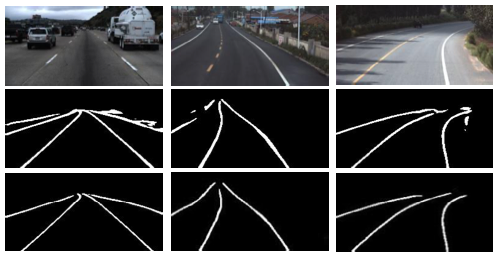
\includegraphics[scale=0.8]{./img/LD_challenging_situations.png}
    \caption{Spurerkennung in unterschiedlichen  Situationen. Erste Reihe: Drei verschiedene Fahrszenen. Zweite Reihe: Erkennung nur anhand des aktuellen Bildes. Dritte Reihe: Spurerkennung anhand des aktuellen und der letzten vier Bilder. \cite[S.1]{cnnld_2020}}
    \label{fig:LDchallenge}
\end{figure}


Es gibt hauptsächlich zwei Arten von Deep Neural Networks. Zum einen \ac{DCNN}, welches Inputdaten häufig mit mehreren Stufen der Convolution verarbeitet und gut geeignet für die Abstraktion von Merkmalen für Bilder und Videos ist. Zum anderen das \ac{DRNN}, das Inputsignale rekursiv verarbeitet, indem es diese in aufeinander folgende Blöcke aufteilt und vollständige Verbindungsschichten für die Statusausbreitung zwischen ihnen aufbaut. Die Vorteile zeigen sich vor allem bei der Vorhersage von Informationen für Zeitreihendaten.\cite{cnnld_2020}


\begin{figure}[H]
    \centering
    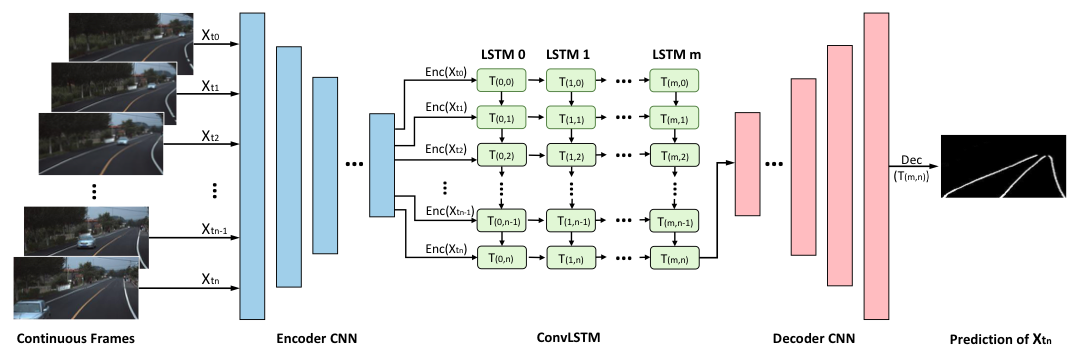
\includegraphics[scale=0.4]{./img/LD_architecture_combined_network.png}
    \caption{Architektur des beschriebenen hybriden Deep Neural Network \cite[S.1]{cnnld_2020}}
    \label{fig:LDHybridDNN}
\end{figure}


Das Team um Qin Zou \cite{cnnld_2020} erhofft sich aus der Kombination eben dieser beiden Netzwerke performante Ergebnisse. So wird ein hybrides Deep Neural Network zur Spurerkennung implementiert. Dabei werden mehrerer kontinuierliche Fahrszenen als Bilder verarbeitet. Das hybride Netzwerk verbindet also die Ansätze von \ac{DCNN} und \ac{DRNN}.
Global betrachtet ist das vorgeschlagene Netzwerk ein \ac{DCNN}, welches mehrere Rahmen als Input verwendet und die Spur des aktuellen Rahmens auf Segmentierungsweise semantisch vorhersagt.
Eine vollständig gefaltete (fully convolution) DCNN-Architektur wird benutzt, um das Segmentierungsziel zu erreichen. Es enthält ein Encoder-Netzwerk und ein Decoder-Netzwerk, diese garantieren, dass die endgültige Ausgabe dieselbe Größe, analog zum Eingabebild hat. Aus der lokalen Perspektive werden vom Encodernetzwerk die von DCNN abstrahierten Merkmale von einem DRNN weiterverarbeitet. Ein \ac{LSTM} Netzwerk wird verwendet, um die Zeitreihen codierter Merkmale zu verarbeiten. Der Output des DRNN führt die Informationen der kontinuierlichen Eingangsrahmen zusammen, welche dann in das Decodernetz des DCNN eingespeist werden, um dann letztendlich die Spuren Vorherzusagen beziehungsweise die Erkennung zu unterstützen. \cite{cnnld_2020}


\subsection{Nutzung Bildmanipulation mithilfe von OpenCV}

Ein weiterer Ansatz ist die Nutzung bildmanipulatorischer Funktionen. Da im Team viel Wissen in diesem Bereich vorherrscht, wurde sich der Datenstrecke von Soumya Ranjan Behera \cite{behera_2019} als grober Anhaltspunkt bedient.
Dabei werden die von einer installierten Kamera gelieferten Inputdaten zuerst in ein Bild aus Grau stufen umgewandelt. Das hat den Vorteil, dass zum einen die zu verarbeitende Datengröße um ein zwei drittel verringert wird. Das schließt sich daraus, dass Bilder im \ac{RGB} Farbraum verarbeitet werden und dieser mit einer Farbtiefe von 0 bis 255 Intensitätspunkten verarbeitet wird. Wenn nun nicht mehr drei Farben mit der gegebenen Farbtiefe, sondern nur eine, also Graustufen, verarbeitet wird, sind es zwei Dimensionen weniger. Dieser Effekt spiegelt sich hauptsächlich in der Verarbeitungszeit der späteren Prozesse wieder.

gaussian_blur

canny

region_of_interest

hough_lines

weighted_img



\section{Implementierung mit OpenCV} %1 Seite


\subsection{Eingangsdaten Vorverarbeitung} %1 Seite


\subection{Canny Edges} %1 Seite1


\subection{Hough Transformation}


\subsection{Verarbeitungsstrecke unter Python}

wichtig ist auch die Geschwindigkeit der Verarbeitung ... in unserem Fall: durchschnittlich 0.06 Sekunden ... wir könnten also an die 1000 Bilder pro Sekunde verarbeiten (gar nicht mal so schlecht)


%Welche Funktionen nutze ich - meine Strecke
- grayscale
    * cv2.cvtColor(img, cv2.COLOR_RGB2GRAY)
- brightness_contrast
    * ImageEnhance.Contrast(img)                [PILLOW funktion]
    * ImageEnhance.Brightness(contrast_img)     [PILLOW funktion]
- gaussian_blur
    * v2.GaussianBlur(img, (kernel_size, kernel_size), 0)
- canny
    * cv2.Canny(img, low_threshold, high_threshold)
- region of interest
    * gets two defined vertices (from get_vertices)
    * the lane polygon has to be set to null values that we can merge the input image and the polygon bitwise
    * done that we add a little polygon to mask the front of the car 
        (to see the car is important for validating the right camera position and a better angle of the lanes)
- hough_lines
    * hough transformation returns a image with the lines
- slope_lines
    * calculate wether a line is left or right and assign to each
    * then print each line
- slope
    * take left and right line of lane and fill it with a color for lane
- weighted_img
- steering


\section{Steuerung} %1 Seiten

